\documentclass{article}

% ---------- Fonts & Encoding ----------
\usepackage[T1]{fontenc}
\usepackage[utf8]{inputenc}
\usepackage{lmodern}
\usepackage{microtype}

% ---------- Math, Figures, Tables ----------
\usepackage{amsmath, amssymb}
\usepackage{graphicx}
\usepackage{booktabs}
\usepackage{multirow}
\usepackage{overpic}
\usepackage{siunitx}

% ---------- Captions ----------
\usepackage{caption}
\usepackage{subcaption}

% ---------- Colors (before hyperref) ----------
\usepackage{xcolor}

% ---------- DLAI Style (optional) ----------
% If the style file exists, load it; otherwise define minimal fallbacks.
\makeatletter
\@ifpackageloaded{dlaiml2025}{}{%
  \IfFileExists{dlaiml2025.sty}{%
    \usepackage[accepted]{dlaiml2025}%
  }{%
    % Minimal fallbacks so the document still compiles without dlaiml2025.
    \newcommand{\dlaititlerunning}[1]{}%
    \newcommand{\dlaititle}[1]{\title{#1}}%
    \newenvironment{dlaiauthorlist}{}{}%
    \newcommand{\dlaiauthor}[2]{}%
  }%
}
\makeatother

\usepackage{hyperref}

\dlaititlerunning{Geodesic Post-Hoc Quantization for VAEs}

\begin{document}

\twocolumn[
\dlaititle{Geodesic Post-Hoc Quantization for Variational Autoencoders}

\begin{dlaiauthorlist}
\dlaiauthor{Marco}{sapienza}
\end{dlaiauthorlist}

\dlaiaffiliation{sapienza}{Sapienza University of Rome}

\dlaicorrespondingauthor{Marco}{galletti.2109043@studenti.uniroma1.it}

\vskip 0.2in
]

\printAffiliationsAndNotice{}

\begin{abstract}
This project revisits the classic VQ-VAE by implementing a post-hoc quantization pipeline. 
Instead of training end-to-end, a continuous-latent VAE is first trained and then a discrete codebook is built by clustering its latent space. This work compares standard graph-based geodesic clustering with two novel variations based on a decoder-induced Riemannian metric. 
Under this metric, latent-space quantization error is reduced by three orders of magnitude, but this does not translate to improved image-space reconstruction quality, where simpler Euclidean-based graph geodesics perform best. 
Furthermore, the success of post-hoc quantization appears to be highly dataset-dependent: 
high-quality results are achieved on structured data like FashionMNIST, but performance degrades on more complex datasets such as CIFAR-10, revealing what appears to be a fundamental trade-off between post-hoc and end-to-end quantization schemes.
\end{abstract}

\section{Introduction}
Generative models, particularly Variational Autoencoders (VAEs), are powerful tools for learning low-dimensional representations of complex data. 
The Vector Quantized VAE (VQ-VAE) extends this by learning a discrete latent space, which is often more suitable for downstream tasks such as autoregressive modeling. 
Standard VQ-VAEs learn this discrete representation end-to-end with the encoder and decoder.
This work explores an alternative post-hoc quantization pipeline, where a continuous-latent VAE is first trained, 
and a discrete codebook is then built by applying clustering algorithms to its latent space.

The main contributions are as follows:
\begin{itemize}
    \item An end-to-end pipeline for post-hoc vector quantization of VAEs.
    \item The implementation and evaluation of a geodesic clustering method based on a decoder-induced Riemannian metric, compared against a standard Euclidean baseline.
    \item A detailed analysis showing that while geodesic clustering better respects the latent manifold's structure, simpler Euclidean clustering consistently yields superior image reconstructions.
    \item The finding that the viability of post-hoc quantization appears to be strongly dependent on dataset complexity, offering insights into the trade-offs between post-hoc and end-to-end learned quantization.
\end{itemize}

The code for this project is available at \url{https://github.com/m4rch1n0/vqvae}.

\section{Related Work}
The project builds upon three main areas of research: discrete latent variable models, the geometric analysis of latent spaces, and graph-based clustering methods.

\paragraph{Discrete Latent Representations.} The Vector-Quantized Variational Autoencoder (VQ-VAE) \cite{van2017neural} is the foundational model for learning discrete representations for generative tasks. 
VQ-VAE introduced the paradigm of learning a discrete codebook end-to-end with the encoder and decoder, and using a powerful autoregressive model over the resulting spatial grid of codes to generate high-fidelity images. 
The research in this project deliberately deviates from this by exploring a post-hoc quantization scheme, which separates the continuous representation learning from the codebook creation.

\paragraph{Geometry of VAE Latent Spaces.} The core motivation for the geodesic method comes from works that model the latent space of a VAE as a Riemannian manifold. Arvanitidis et al. \cite{arvanitidis2017latent} established the use of the pull-back metric tensor, defined by the decoder's Jacobian ($M(z) = J(z)^T J(z)$), to better represent the geometry of the data manifold. They argued for using geodesic distances, rather than Euclidean ones, for tasks like interpolation and clustering. Shao et al. \cite{shao2018riemannian} further developed practical methods for geodesic computation, though they noted that for some image VAEs, the learned manifolds can be nearly flat, making Euclidean distance a reasonable approximation. 
This work leverages these geometric insights directly, using Jacobian-vector product to approximate local geodesic distances for clustering.

\paragraph{Graph-Based Geodesic Approximation.} The specific technique of approximating geodesic distances by computing shortest paths on a k-Nearest Neighbors (k-NN) graph was popularized by Isomap \cite{tenenbaum2000global} in the context of manifold learning. This approach provides a computationally feasible way to estimate global manifold distances from local neighborhood information. The methods presented here are a direct application of this principle: a k-NN graph is constructed and shortest-path distances (via Dijkstra's algorithm) are used as the metric for the k-medoids clustering algorithm, with the key novelty being the re-weighting of the graph's edges with the learned Riemannian metric.

\section{Method}
The pipeline consists of three main stages: continuous representation learning, post-hoc quantization, and autoregressive modeling.

\subsection{Model Architectures\protect\footnote{Model implementations are available at \texttt{vqvae/src/models/$\footnotesize\{\texttt{spatial\_vae.py}, \texttt{transformer.py}\}$.}}}
\paragraph{Spatial VAE.} The VAE encoder consists of three convolutional layers (with 64, 128, and 256 channels respectively, stride 2, and Batch Normalization) that downsample the input image to a $4 \times 4$ spatial grid. 
Two final $1 \times 1$ convolutions produce the mean and log-variance for a latent space at each spatial location (16-dim for FashionMNIST, 32-dim for CIFAR-10). The decoder mirrors this architecture using transposed convolutions to reconstruct the image.

\paragraph{Transformer.} A decoder-only Transformer is used for autoregressive modeling of the quantized latent codes. For both datasets, the model has 4 layers, 4 attention heads, an embedding dimension of 256, and is trained on flattened $16$-token sequences.

\subsection{Training Details}
The \texttt{SpatialVAE} for both datasets was trained for 200 epochs using the AdamW optimizer with a learning rate of $10^{-3}$, a weight decay of $10^{-5}$, and a cosine learning rate schedule. 
The Transformer models were also trained for 200 epochs with AdamW, but with a learning rate of $3 \times 10^{-4}$ and a weight decay of $0.01$. The batch size for all experiments was 256.

\subsection{Post-Hoc Quantization Methods}
After training a VAE, the mean latent vectors ($\mu$) are extracted from the training set and a discrete codebook is built by clustering this latent space. 
The analysis on FashionMNIST compares three distinct graph-based quantization schemes which progressively incorporate the learned manifold geometry.

\paragraph{Method 1: Graph Geodesic Clustering.}
This baseline clustering method first constructs a k-NN graph from the latent vectors, with edge weights defined by the standard Euclidean distance. 
K-medoids clustering is then performed, where the distance between any two points on the graph is calculated as the shortest path between them (a "graph geodesic"). 
This method was applied to the latent space of the \texttt{vanilla VAE}.

\paragraph{Method 2: Partial Riemannian Geodesic Clustering.}
This method aims to improve upon the first by incorporating the VAE's learned geometry. 
It begins with the same Euclidean-weighted k-NN graph, but then re-weights a small, stratified subset of the edges (5,000 by default) using the decoder-induced Riemannian metric described in the introduction. 
Clustering is then performed on this hybrid graph, which is mostly Euclidean but is locally corrected by the Riemannian metric. This was also applied to the latent space of the \texttt{vanilla VAE}.
\paragraph{Method 3: Full Riemannian Geodesic Clustering.}
This is the most geometrically rigorous approach. It re-weights \textit{all} unique edges in the k-NN graph with the Riemannian metric. The subsequent k-medoids clustering is therefore performed on a graph that fully represents the learned manifold structure. This method was applied to the latent space of a \texttt{SpatialVAE}, which represents a change in the underlying VAE architecture as well as the quantization scheme.

\subsection{Autoregressive Modeling}
Once the codebook is built, the spatial latent grids for each training image are quantized, converting them into sequences of discrete integer codes. A decoder-only Transformer model is then trained to predict the next code in a sequence, \textbf{conditioned on the previous ones}. This allows for autoregressive generation of novel sequences of codes, which can then be mapped back to latent vectors via the codebook and rendered into images by the VAE decoder.

\section{Experiments and Results}
The pipeline was evaluated on two datasets of varying complexity: FashionMNIST and CIFAR-10.
Performance was assessed using Peak Signal-to-Noise Ratio (PSNR) and Structural Similarity Index (SSIM).
\subsection{Comparative Analysis on FashionMNIST}
The primary analysis compares the three quantization methods on the FashionMNIST dataset. 
As shown in Table~\ref{tab:fashion_mnist_results}, the results suggest a nuanced trade-off between geometric accuracy and reconstruction quality. The graph geodesic method with pure Euclidean weights achieves the highest performance. The introduction of a partial Riemannian correction provides a competitive result, while the full Riemannian method, though most geometrically faithful, yields a lower reconstruction quality.

\begin{table}[h!]
\caption{FashionMNIST Quantization Method Comparison.\protect\footnotemark}
\label{tab:fashion_mnist_results}
\begin{center}
\begin{footnotesize}
\begin{tabular}{l c c}
\toprule
Method & PSNR (dB) & SSIM \\
\midrule
Graph Geodesic (Euclidean) & \textbf{33.42} & \textbf{0.9589} \\
Partial Riemannian Geodesic & 31.95 & 0.9432 \\
Full Riemannian Geodesic & 9.84 & 0.5168 \\
\bottomrule
\end{tabular}
\end{footnotesize}
\end{center}
\vspace{-0.4cm}
\end{table}
\footnotetext{Metrics are computed consistently across all methods. While absolute values may be implementation-dependent, the relative performance ranking is valid.}

\begin{figure*}[!p]
    \centering
    \begin{subfigure}[b]{0.32\textwidth}
        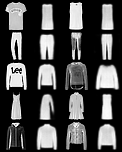
\includegraphics[width=\linewidth]{images/fashion_vanilla_euclidean_comparison_grid.png}
        \caption{Method 1: Graph Geodesic (Euclidean)}
        \label{fig:euclidean_recon}
    \end{subfigure}
    \hfill
    \begin{subfigure}[b]{0.32\textwidth}
        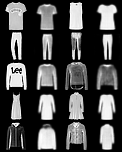
\includegraphics[width=\linewidth]{images/fashion_vanilla_geodesic_comparison_grid.png}
        \caption{Method 2: Partial Riemannian Geodesic}
        \label{fig:partial_recon}
    \end{subfigure}
    \hfill
    \begin{subfigure}[b]{0.32\textwidth}
        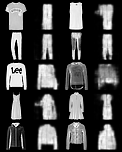
\includegraphics[width=\linewidth]{images/fashion_spatial_geodesic_comparison_grid.png}
        \caption{Method 3: Full Riemannian Geodesic}
        \label{fig:full_recon}
    \end{subfigure}
    \caption{Qualitative comparison of FashionMNIST reconstructions from the three different post-hoc quantization methods. In each subfigure, the top row shows original images and the bottom row shows their reconstructions. The visual quality directly corresponds to the quantitative results in Table 1, with the Euclidean-based method producing the sharpest images and the Full Riemannian method showing significant degradation.}
    \label{fig:fashion_recon}
\end{figure*}

\subsection{CIFAR-10: Post-Hoc vs. End-to-End Training}
For the more complex CIFAR-10 dataset, the analysis was focused on comparing our strongest post-hoc method (Full Riemannian Geodesic on a Spatial VAE) against a baseline, end-to-end trained VQ-VAE. The results, summarized in Table~\ref{tab:cifar10_results}, suggest the superiority of the end-to-end approach. The baseline VQ-VAE outperforms the post-hoc method across all key metrics, including reconstruction quality (PSNR, SSIM) and perceptual similarity (LPIPS). This suggests the importance of jointly training the encoder, decoder, and codebook on complex data distributions.

\begin{table}[h!]
\caption{CIFAR-10 Method Comparison.\protect\footnotemark}
\label{tab:cifar10_results}
\begin{center}
\begin{footnotesize}
\begin{tabular}{l c c c}
\toprule
Method & PSNR (dB) & SSIM & LPIPS \\
\midrule
Post-Hoc (Full Riemannian) & 8.72 & 0.005 & 0.564 \\
Baseline VQ-VAE & \textbf{9.49} & \textbf{0.019} & \textbf{0.475} \\
\bottomrule
\end{tabular}
\end{footnotesize}
\end{center}
\vspace{-0.4cm}
\end{table}
\footnotetext{Metrics are computed consistently across all methods. While absolute values may be implementation-dependent, the relative performance ranking is valid.}

\begin{figure*}[!p]
    \centering
    \begin{subfigure}[b]{0.32\textwidth}
        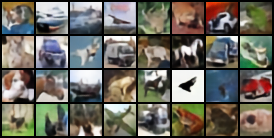
\includegraphics[width=\linewidth]{images/cifar10_baselineVQ.png}
        \caption{Baseline VQ-VAE (Reconstructions)}
        \label{fig:cifar_baseline}
    \end{subfigure}
    \hfill
    \begin{subfigure}[b]{0.32\textwidth}
        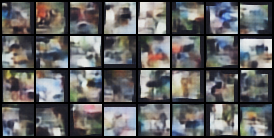
\includegraphics[width=\linewidth]{images/cifar10_spatial_geodesic_generated_samples.png}
        \caption{Post-Hoc Spatial Geodesic (Generated)}
        \label{fig:cifar_spatial}
    \end{subfigure}
    \hfill
    \begin{subfigure}[b]{0.32\textwidth}
        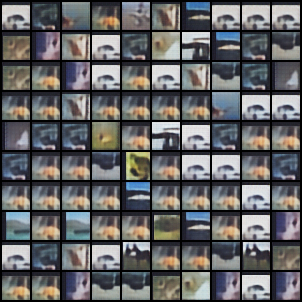
\includegraphics[width=\linewidth]{images/cifar10_vanilla_euclidean_generated_samples.png}
        \caption{Post-Hoc Vanilla Euclidean (Generated)}
        \label{fig:cifar_vanilla}
    \end{subfigure}
    \caption{Qualitative comparison on CIFAR-10. (a) Reconstructions from the end-to-end baseline VQ-VAE are coherent and recognizable. (b) Samples generated by the Transformer in the post-hoc spatial geodesic pipeline are less coherent. (c) Samples from the post-hoc vanilla pipeline show clear signs of mode collapse, where the model repeatedly generates the same limited set of outputs, failing to capture the data diversity.}
    \label{fig:cifar_recon}
\end{figure*}

\section{Discussion and Conclusions}
FashionMNIST results show that while Riemannian metrics achieve more geometrically faithful clustering (quantization error $3.40 \times 10^5$ vs. Euclidean's $3.55 \times 10^8$), this does not translate to superior image reconstruction. Latent-space distortion metrics do not perfectly correlate with image-space metrics like PSNR. Best performance comes from simple graph-geodesic clustering with Euclidean weights.

The partial Riemannian method suggests that limited application of the Riemannian metric may act as regularization, correcting local geometry without being dominated by noise in the fully-reweighted manifold. However, the full Riemannian method was tested on a \texttt{SpatialVAE} while others used vanilla VAE - an architectural confound requiring future work.

On CIFAR-10, the "training mismatch" in post-hoc methods creates a performance bottleneck overcome by joint, end-to-end optimization of standard VQ-VAE.

In conclusion, this project reveals a complex trade-off between geometric fidelity and reconstruction performance. While leveraging a decoder-induced Riemannian metric substantially reduces latent-space quantization error, this geometric accuracy does not translate to improved image quality. On FashionMNIST, simpler graph-geodesic methods with Euclidean weights outperformed more rigorous Riemannian approaches. On CIFAR-10, the "training mismatch" of post-hoc frameworks proved a significant bottleneck, with end-to-end trained VQ-VAE achieving superior results. Future work could address this by fine-tuning the decoder on discrete codebooks, combining benefits of geometric clustering with jointly-optimized performance.

\bibliography{references.bib}
\bibliographystyle{dlaiml2025}

\end{document}
